% HW3 high dimensional data

\documentclass[12pt, leqno]{article}
\usepackage{amsfonts, amsmath, amssymb}
\usepackage{amsthm}
\usepackage{mathtools}
\usepackage{fancyhdr}
\usepackage{hyperref}
\usepackage{graphicx}
\usepackage{caption}
\usepackage{subcaption}
\usepackage{float}
\usepackage{mathrsfs}
\usepackage{array} 
\usepackage{rotating}
\usepackage{rotating}
\usepackage{booktabs}
\usepackage{bbm}
%\usepackage{babel}
\providecommand{\abs}[1]{\lvert#1\rvert}
\providecommand{\norm}[1]{\lVert#1\rVert}
\newcommand{\macheps}{\epsilon_{\mbox{\scriptsize mach}}}
\let\oldhat\hat
\renewcommand{\vec}[1]{\mathbf{#1}}
\renewcommand{\hat}[1]{\oldhat{{#1}}}
\def\rp{\ensuremath \mathbb{R}^p}
\def\rpp{\ensuremath \mathbb{R}^{p \times p}}
\def\s{\ensuremath\Sigma}
\def\om{\ensuremath\Omega}
\def\pd{\ensuremath\mathbb{P}^+}
\def\pg{\ensuremath\mathbb{P}_{{G}}}
\def\E{\ensuremath\mathbb{E}}
\def\normdist[#1]#2{\ensuremath \sim \mathcal{N} (#1,#2) }
\def\ndist1{\ensuremath \sim \mathcal{N}  (\mu, \sigma)}
\def\ndistvec{\ensuremath \sim \mathcal{N}_p ( {\mu},  {\Sigma})}
\def\lra{\ensuremath\Leftrightarrow}
\def\stackrel#1#2{\mathrel{\mathop{#2}\limits^{#1}}}
\newcommand\ind{\protect\mathpalette{\protect\independenT}{\perp}}
\def\independenT#1#2{\mathrel{\rlap{$#1#2$}\mkern2mu{#1#2}}}
\makeatletter
\newtheorem{thm}{Theorem}[]
\newtheorem{lemma}{Lemma}[]
\newtheorem{defn}[thm]{Definition}
\newcommand{\sign}{\mathrm{sign}}
\newcommand{\prox}{\mathrm{prox}}
\newcommand{\trace}{\mathrm{trace}}
\newcommand{\diag}{\mathrm{diag}}
\newcommand{\distas}[1]{\mathbin{\overset{#1}{\kern\z@\sim}}}%
\newsavebox{\mybox}\newsavebox{\mysim}
\newcommand{\dist}[1]{%
  \savebox{\mybox}{\hbox{\kern3pt$\scriptstyle#1$\kern3pt}}%
  \savebox{\mysim}{\hbox{$\sim$}}%
  \mathbin{\overset{#1}{\kern\z@\resizebox{\wd\mybox}{\ht\mysim}{$\sim$}}}%
}
\makeatother

\begin{document}
\pagestyle{fancy}
\lhead{Syed Rahman}
\rhead{STA7934}

\begin{center}
{\large {\bf Take Home Final - Analysis of High Dimensional Data}} \\
\end{center}

\paragraph{1a.} Let $f(x) = \norm{x}_1$ with domain of $f =
\{x:\norm{x}_{\infty} \leq 1\}$. 
Note that 
\begin{align*}
  [\prox_{f}(x)]_i &= \arg\min_{u}[(\norm{u}_1 + \frac{1}{2} \norm{u-x}_2^2)]_i\\
  &= \begin{cases} x_i-1 & \text{ if } x_i>1 \\
0 & \text{ if } \abs{x_i} \leq 1 \\
x_i + 1 & \text{ if } x_i<-1
\end{cases}
\end{align*}
Now for $\prox_{f}(x)$ such that $\{u:\norm{u}_{\infty} \leq 1\}$ we
will have  
\begin{align*}
  [\prox_{f}(x)]_i 
  &= \begin{cases} 1 &  \text{ if } x_i>2 \\
x_i - 1 & \text{ if } 1< x_i \leq 2 \\
0 & \text{ if } \abs{x_i} \leq 1 \\
x_i + 1 & \text{ if } -2 \leq x_i<-1 \\
-1 &\text{ if }  x_i<-2 
\end{cases}
\end{align*}

\paragraph{1b.} Let $f(x) = \max_{k=1,...,n} x_k = \norm{x}_{\infty}$.
Thus 
\begin{align*}
\prox_{f} (x) &= \arg\min_{u} (\norm{u}_{\infty} +
               \frac{1}{2}\norm{u-x}_2^2) \\
&= x - P_C(x)
\end{align*}
where $C = \{x|\norm{x}_1 \leq 1\}$.
Note that 
\begin{align*}
[P_C(x)]_i =   &= \begin{cases} x_i-\lambda & \text{ if } x_i>\lambda \\
0 & \text{ if } \abs{x_i} \leq \lambda \\
x_i + \lambda & \text{ if } x_i<-\lambda
\end{cases}
\end{align*}
where $\lambda = 0$ if $\norm{x}_1 \leq 1$ and otherwise is the
solution of the equation 
\[
\sum_{i=1}^n \max\{\abs{x_i}-\lambda,0\} = 1.
\]

\paragraph{1c.} Let $f(x) = \norm{Ax-b}_1$ where $AA' = D = \diag(d_{11},...,d_{pp})$.
Thus 
\begin{align*}
\prox_{f} (x) &= \arg\min_{u} (\norm{Au-b}_{1} +
               \frac{1}{2}\norm{u-x}_2^2) \\
&= \arg\min_{y,u} (\norm{y}_{1} +
               \frac{1}{2}\norm{u-x}_2^2) \text { subject to } Au-b = y\\
\end{align*} 
Note that as $AA' = D$, 
\[
Av = \begin{cases} 
d & \text{ if } v \in \mathcal{C}(A')\\ 
0 & \text{ if } v \not\in \mathcal{C}(A')\\ 
\end{cases}
\]
Thus for $u-x \in \mathcal{C}(A')$ 
\begin{align*}
u-x &= A'(AA')^{-1}A(u-x) \\ 
&= A'(AA')^{-1}(y+b-Ax)\\
\implies \prox_{f} (y) &= \arg\min_{y}(\norm{y}_{1} +
                         \frac{1}{2}\norm{A'(AA')^{-1}(y+b-Ax)}_2^2)
  \\
&=\arg\min_{y}(\norm{y}_{1} +
                         \frac{1}{2}\norm{D^{-\frac{1}{2}}(y+b-Ax)}_2^2)
  \\
&= \arg\min_{y}(\sum_{i=1}^p \abs{y_i} + \frac{1}{2 {d_{ii}}}(y_i
  + b_i - a_i'x)^2) \\
&= \arg\min_{y}(\sum_{i=1}^p {d_{ii}} \abs{y_i} + \frac{1}{2}(y_i
  + b_i - a_i'x)^2) \\
\implies   [\prox_{f}(y)]_i 
  &= \begin{cases}  -(b_i - a_i'x) - {d_{ii}}&  \text{ if } -(b_i - a_i'x)>{d_{ii}} \\
0 & \text{ if } \abs{-(b_i - a_i'x)} \leq {d_{ii}} \\
 -(b_i - a_i'x) + {d_{ii}} & \text{ if }  -(b_i - a_i'x) < -{d_{ii}}
\end{cases}
\end{align*}

\paragraph{1d.} For this problem, for $\s = PDP' \in S_{++}^n$,
$\s ^{\frac{1}{2}} = PD^{\frac{1}{2}}P'$. 

Let $f(X) = -\log \det(X), X \in S_{+}^n$ and domain$(f) =
S_{++}^n$.
\begin{align*}
\prox_f(X) &= \arg\min_{U}(-\log \det(U) + \frac{1}{2}\norm{U-X}_F^2)
  \\
&= \arg\min_{U}(-\log \det(U) + \frac{1}{2}\trace(U-X)(U-X)') 
\end{align*}
Note that
\begin{align*}
\frac{d}{dU} (\log \det(U)) &=  \frac{1}{\det(U)} \frac{d}{dU} \det(U)
\\
&=  \frac{1}{\det(U)} \det(U) (U^{-1}) \\
&=  U^{-1}
\end{align*}
and
\begin{align*}
\frac{d}{dU} \trace(U-X)(U-X)') &= 2U - 2X
\end{align*}
which implies that
\begin{align*}
\frac{d}{dU} (-\log \det(U) + \frac{1}{2}\trace(U-X)(U-X)') &=
                                                              -U^{-1}
                                                              + U -
                                                              X  =
                                                              0\\
\iff -I + U^2 - UX = 0 \\
\iff   U^2 - UX = I \\
\iff   U^2 - 2U(\frac{1}{2}X) +(\frac{1}{2}X)^2 = I +(\frac{1}{2}X)^2
  \\
\iff   (U -(\frac{1}{2}X))^2 = I +(\frac{1}{2}X)^2 \\
\iff   U -(\frac{1}{2}X) = (I +(\frac{1}{2}X)^2)^{\frac{1}{2}} \\
\iff   U = (I +(\frac{1}{2}X)^2)^{\frac{1}{2}}  + (\frac{1}{2}X) \succ 0.
\end{align*}
Thus
\begin{align*}
\prox_f(X) &= (I +(\frac{1}{2}X)^2)^{\frac{1}{2}}  + (\frac{1}{2}X).
\end{align*}


\paragraph{2} We want to solve the following problem:
\begin{align*}
\textbf{Primal:}&\min (x_1 - x_2) \\
&\text{subject to } x \in X = \{x:x_1 \geq 0, x_2 \geq 0\}, x_1+1 \leq
  0, 1 - x_1 - x_2 \leq 0
\end{align*}
Now the Lagrangian is 
\begin{align*}
\mathcal{L}(x,\lambda) &= (x_1 - x_2) + \lambda_1(-x_1) +
                         \lambda_2(-x_2) \\
&\quad + \lambda_3(x_1+1) + \lambda_4(1 - x_1 - x_2) \\
&= x_1(1-\lambda_1+\lambda_3-\lambda_4) + x_2(-1 - \lambda_2 -
  \lambda_4) + \lambda_3 + \lambda_4 \\
\implies g(\lambda_1,\lambda_2,\lambda_3,\lambda_4) &=
                                                      \inf_{x}\mathcal{L}
                                                      (x,\lambda) \\
&= \begin{cases} -\infty & \text{ if } 1-\lambda_1+\lambda_3-\lambda_4
  \not= 0 \text { or } -1 - \lambda_2 -
  \lambda_4 \not= 0 \\
\lambda_3 + \lambda_4 & \text{ else }
\end{cases}
\end{align*}
Thus the dual problem is 
\begin{align*}
\textbf{Dual:}&\max_{\lambda_i \geq 0} \lambda_3 + \lambda_4 \\
&\text{subject to } 1-\lambda_1+\lambda_3-\lambda_4
  = 0 \\
& \text {and } -1 - \lambda_2 -
  \lambda_4 = 0
\end{align*}
The constraints have
infinitely many solutions. Hence this is clearly maximized when
$\lambda_i = \infty, i = 3,4$ which implies that the
dual is unbounded. 

\paragraph{3a.} Let $A_j \in \mathbb{R}^{m \times n}, y_j \in
\mathbb{R}$. We want to solve the following problem: 
\begin{align*}
\textbf{Primal:}&\min_{X \in \mathbb{R}^{m \times n}} \sum_{j = 1}^J
                  (y_j - \trace (X'A_j))^2 \\
&\text{subject to } \norm{X}_* \leq t
\end{align*}
or equivalently,
\begin{align*}
\min_{X \in \mathbb{R}^{m \times n}} \sum_{j = 1}^J
                  (y_j - \trace (X'A_j))^2 + \lambda \norm{X}_*
\end{align*} 
For our simulations we used, $m = 10,n = 5$ and $J = 5$. In addition,
$A_j$ are matrices with elements randomly generated from
$\mathcal{U}(-5,5)$. To generate the true $X$ we generated a matrix
with elements from $\mathcal{U}(-5,5)$ took the $SVD$ as $U \s V'$ and set
$X = UV'$. We then calculated $y_j =  \trace (X'A_j) +
\epsilon_j$ where $\epsilon_j \sim \mathcal{N}(0,1)$. 
Note that $\frac{d}{dX} \sum_{j = 1}^J
                  (y_j - \trace (X'A_j))^2 = -2 \sum_{j = 1}^J(y_j -
                  \trace (X'A_j))A_j$.
Thus a proximal gradient method would be
\begin{align}
X^{k+1} &= X^{k} + t(2 \sum_{j = 1}^J(y_j -
                  \trace ((X^k)'A_j))A_j) \\
X^{k+1} &= S_{t\lambda}(X^{k+1})
\end{align}
where $t$ is the stepsize and $S_{t\lambda}(X^{k+1}) =
 U S_{t\lambda}(\s) V'$. Here, 
\begin{align*}
X &= U \s V' \\ 
&= U \diag(\sigma_1,...,\sigma_p) V' 
\end{align*} 
is the SVD of $X$ and $S_{t\lambda}(\s) =
\diag(S_{t\lambda}(\sigma_1),...,S_{t\lambda}(\sigma_p))$ is the soft
thresholding operator applied elementwise to the diagonal of $\s$.
Using a cross-validation procedure we find that $\lambda \approx 570$
minimizes the objective function as shown in Figure \ref{fig:no3cv}. Doing 10 replications using this
value of $\lambda$ converges in about $200-300$ iterations and gives
us an average Frobenius norm loss of
\[
F = \sum_{r = 1}^{10}\frac{\norm{\hat{X}_r-X_r}_F}{\norm{X_r}_F} =   0.9858716.
\]
We define relative error as 
\[
RE = \frac{\norm{\hat{X}^k-X_{true}}_F}{\norm{X_{true}}_F}
\]
This is shown in Figure \ref{fig:no3error} for $\lambda = 570$.

In general as $m,n$ and $J$ increase we need to reduce the stepsize
to achieve convergence. For $m = 50,n=30, J = 100$ and $\lambda = 100$ with a
stepsize of $10^{-7}$ we achieved convergence in $200-300$ iterations
with an average Frobenius norm loss of 
\[
F = \sum_{r = 1}^{10}\frac{\norm{\hat{X}_r-X_r}_F}{\norm{X_r}_F} =   1.001247.
\]
\begin{figure}
\begin{center}
                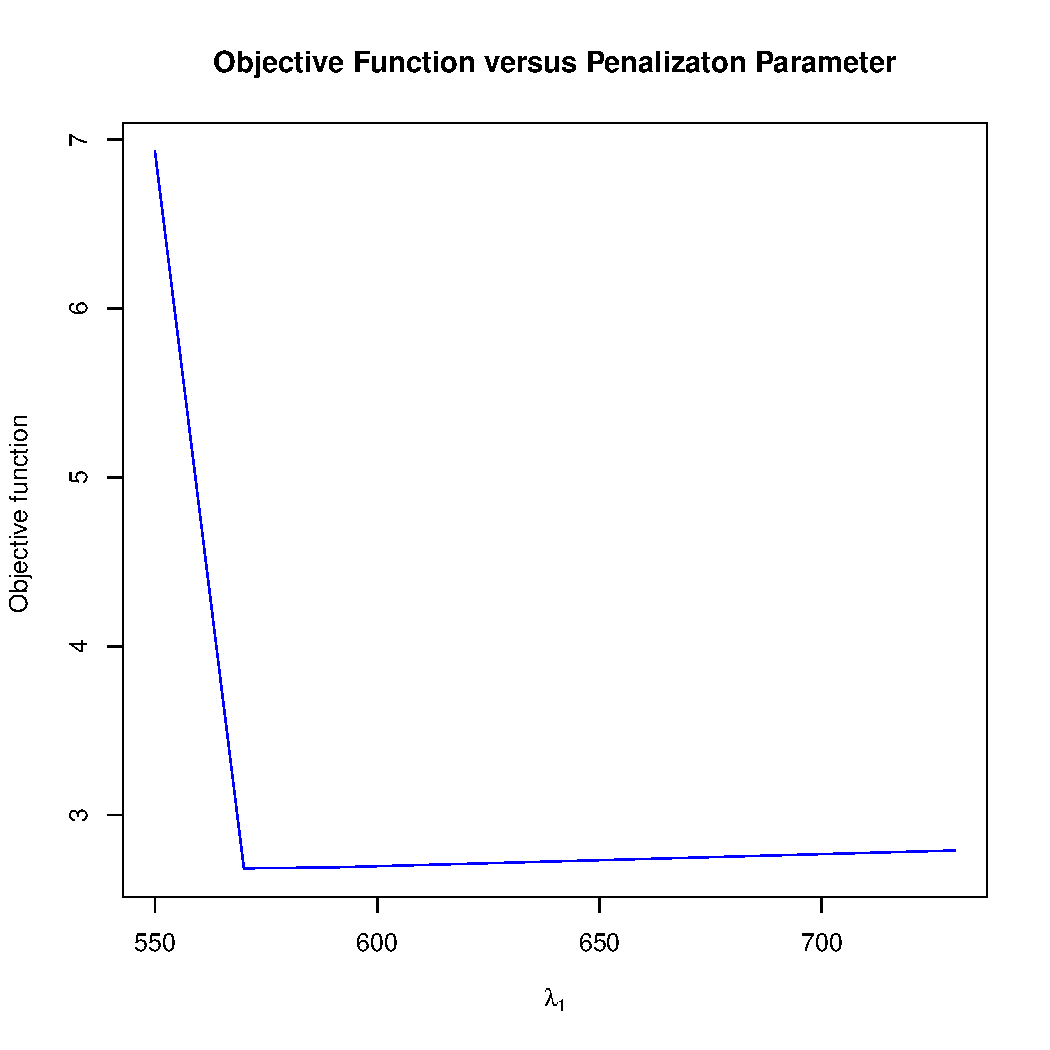
\includegraphics[scale = 0.4]{takehome3cv.pdf}
                \caption{Value of objective function for predicted $X_{\lambda}$ versus $\lambda$ for trace norm
                  constrained optimization problem}
                \label{fig:no3cv}
\end{center}
\end{figure}

\begin{figure}
\begin{center}
                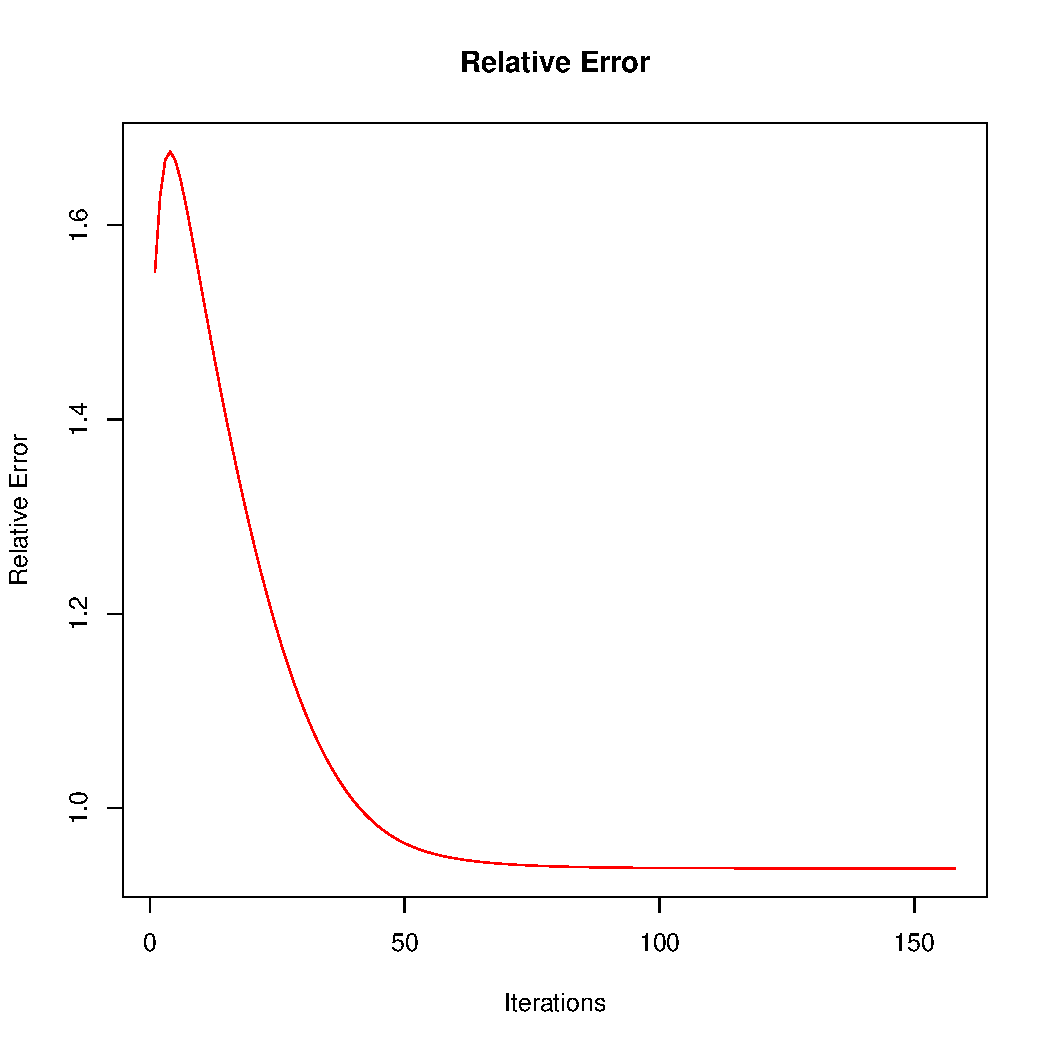
\includegraphics[scale = 0.4]{takehome3error.pdf}
                \caption{Relative Error plot for trace norm
                  constrained optimization problem}
                \label{fig:no3error}
\end{center}
\end{figure}

\paragraph{4.} We propose two methods to solve this problem.
We want to solve the following problem for $i = 1,...,p$:
\begin{align*} \textbf{Method 1:}
&\min \norm{\beta^{1}}_1 + \norm{\beta^{2}}_1 + \norm{\beta^{2} -\beta^{1}}_1\\
&\text{subject to } \norm{S\beta^{1} - e_i}_{\infty} \leq t_1 ,
  \norm{S\beta^{2} - e_i}_{\infty} \leq t_2 
\end{align*}
Note that this is equivalent to
\begin{align*}
&\min \norm{\beta^{1}}_1 + \norm{\beta^{2}}_1 + \norm{\beta^{2} -\beta^{1}}_1\\
&\text{subject to } - t_11 \leq S\beta^{1} - e_i\leq t_11 \\
&\text{and }  -t_21 \leq S\beta^{2} - e_i \leq t_21 \\
\end{align*}
Now reparametrize by letting $u_j^1 = \abs{\beta_j^{1}}_1$, $u_j^2 =
\abs{\beta_j^{2}}_1$ and $z_j = \abs{\beta_j^2 - \beta_j^1}$. Then the problem is 
\begin{align*}
&\min \sum_{j = 1}^p{u_j^1} +  \sum_{j = 1}^p{u_j^2} + \sum_{j = 1}^p{z_j} \\
&\text{subject to } -\beta^{1} \leq u^1 \leq \beta^{1},-\beta^{2} \leq
  u^2 \leq \beta^{2} \\
&\text{ and } \beta^{1}-\beta^{2} \leq z \leq \beta^{2} - \beta^{1}\\
&\text{ and } - t_11 \leq S\beta^{1} - e_i\leq t_11 \\
&\text{and }  -t_21 \leq S\beta^{2} - e_i \leq t_21 
\end{align*}
Hence we can write the above problem as a linear programming problem:
\begin{align*}
&\min c^Tx \\
&\text{subject to } Ax \leq b \\
&\text{and } x \geq 0
\end{align*}
where 
\[
x = \begin{pmatrix} u^1 \\u^2 \\\beta^{1} + u^1 \\ \beta^{2} + u^2 \\z \end{pmatrix},
\]
\[
c^T = \begin{pmatrix} 1 &1&0&0&1 \end{pmatrix},
\]
\[
A = \begin{pmatrix} 
-2I&0&I&0&0\\
0&0&-I&0&0\\
0&-2I&0&I&0\\
0&0&0&-I&0\\
-S&0&S&0&0\\
S&0&-S&0&0\\
0&-S&0&S&0\\
0&S&0&-S&0\\
I&-I&-I&I&-I\\
I&-I&-I&I&I
\end{pmatrix},
\]
and
\[
b^T = \begin{pmatrix}
  0&0&0&0&t_11+e_i&t_11-e_i&t_21+e_i&t_21-e_i&0&0 \end{pmatrix}.
\]
For the second method we want to solve the following problem for $i = 1,...,p$:
\begin{align*} \textbf{Method 2:}
&\min \norm{\beta^{1}}_1 + \norm{\beta^{2}}_1 \\
&\text{subject to } \norm{S\beta^{1} - e_i}_{\infty} \leq t_1 ,
  \norm{S\beta^{2} - e_i}_{\infty} \leq t_2 \\
&\text{ and } \norm{\beta^{2} - \beta^{1}}_{\infty} \leq t_3
\end{align*}
Note that this is equivalent to
\begin{align*}
&\min \norm{\beta^{1}}_1 + \norm{\beta^{2}}_1 \\
&\text{subject to } - t_11 \leq S\beta^{1} - e_i\leq t_11 \\
&\text{and }  -t_21 \leq S\beta^{2} - e_i \leq t_21 \\
&\text{ and } -t_31 \leq \beta^{2} - \beta^{1} \leq t_31
\end{align*}
Now reparametrize by letting $u^1 = \abs{\beta^{1}}_1$ and $u^2 =
\abs{\beta^{2}}_1$. Then the problem is 
\begin{align*}
&\min \sum_{j = 1}^p{u_j^1} +  \sum_{j = 1}^p{u_j^2} \\
&\text{subject to } -\beta^{1} \leq u^1 \leq \beta^{1},-\beta^{2} \leq
  u^2 \leq \beta^{2} \\
&\text{ and } - t_11 \leq S\beta^{1} - e_i\leq t_11 \\
&\text{and }  -t_21 \leq S\beta^{2} - e_i \leq t_21 \\
&\text{ and } -t_31 \leq \beta^{2} - \beta^{1} \leq t_31
\end{align*}
or equivalently,
\begin{align*}
&\min \sum_{j = 1}^p{u_j^1} +  \sum_{j = 1}^p{u_j^2} \\
&\text{subject to } 0 \leq 2u^1 + (\beta^{1}-u^1) \leq 2 \beta^{1},0 \leq 2u^2+
  (\beta^{2}-u^2) \leq 2\beta^{2} \\
&\text{ and } S(\beta^{1} + u^1) - Su^1\leq e_i + t_11 \\
&\text{ and }  - (S(\beta^{1} + u^1) - Su^1)  \leq t_11 - e_i \\
&\text{ and } S(\beta^{2} + u^2) - Su^2 \leq e_i + t_21 \\
&\text{ and }  - (S(\beta^{2} + u^2) - Su^2)  \leq t_21 - e_i \\
&\text{ and } (\beta^{1} - u^1) - (\beta^{2} - u^2) + u^1 - u^2 \leq -t_31 \\
&\text{ and } (\beta^{2}-u^2)- (\beta^{1}-u^1) - u^1 + u^2\leq t_31 \\
\end{align*}
Hence we can write the above problem as a linear programming problem:
\begin{align*}
&\min c^Tx \\
&\text{subject to } Ax \leq b \\
&\text{and } x \geq 0
\end{align*}
where 
\[
x = \begin{pmatrix} u^1 \\u^2 \\\beta^{1} + u^1 \\ \beta^{2} + u^2 \end{pmatrix},
\]
\[
c^T = \begin{pmatrix} 1 &1&0&0 \end{pmatrix},
\]
\[
A = \begin{pmatrix} 
-2I&0&I&0\\
0&0&-I&0\\
0&-2I&0&I\\
0&0&0&-I\\
-S&0&S&0\\
S&0&-S&0\\
0&-S&0&S\\
0&S&0&-S\\
I&-I&-I&I\\
-I&I&I&-I\\
\end{pmatrix},
\]
and
\[
b^T = \begin{pmatrix}
  0&0&0&0&t_11+e_i&t_11-e_i&t_21+e_i&t_21-e_i&t_31&-t_31 \end{pmatrix}.
\]
For both methods set $\hat{\beta}^1 = (\hat{\beta}^1+\hat{u}^1) - \hat{u}^1$ and
$\hat{\beta}^2 = (\hat{\beta}^2+\hat{u}^2) - \hat{u}^2$ and let the solutions
to the $i$-th problem be the $i$-th columns of
$\hat{\om}^1$ and $\hat{\om}^2$. Finally we symmetrized $\hat{\om}^k$
by taking $\hat{\om}^k_{ij} = \min(\hat{\om}^k_{ij},\hat{\om}^k_{ji})$
as reccomended by Cai et. al (2011). For method 1, we tried values of $t_1= t_2$ from a
grid between 0.05 and 0.95 and settled on 0.1 as that minimized the
distance between the false positive and false negative rates for the
values we tried. We tried a similar approach for method 2, except that
we first searched for the optimal $t1=t2$ and then for $t3$.

For both $\om^1$ and $\om^2$ we calculate the following statistics. 
\begin{align*}
F (\hat{\om}) &=\frac{1}{20} \sum_{k=1}^{20}
                \frac{\norm{\om^{(k)}-\hat{\om^{(k)}}}_F^2}{\norm{\om^{(k)}}_F^2}\\
F_{mle} (\hat{\om}) &=\frac{1}{20} \sum_{k=1}^{20} \frac{\norm{\om_{mle}^{(k)}-\hat{\om^{(k)}}}_F^2}{\norm{\om^{(k)}}_F^2}\\
FP (\hat{\om}) &= \frac{1}{20} \sum_{k=1}^{20}\frac{\sum_{i,j} I(\omega^{(k)}_{ij}=0,\hat{\omega}^{(k)}_{ij}\not=0)}{\sum_{i,j} I(\omega^{(k)}_{ij}=0)}\\
FN (\hat{\om}) &= \frac{1}{20} \sum_{k=1}^{20} \frac{\sum_{i,j}
     I(\omega^{(k)}_{ij}\not=0,\hat{\omega}^{(k)}_{ij}=0)}{\sum_{i,j}
     I(\omega^{(k)}_{ij}\not=0)}
\end{align*}

Note that $F_{mle}$ was calculated by finding the corresponding graph first and
then solving the following problem:
\begin{align} \label{eq:glasso}
&\max_{\om \succ 0} \log\abs{\om}-tr(\om S) \\
&\text{ subject to } (i,j) \not\in E \implies \omega_{ij} = 0. \nonumber
\end{align}
In the tables below we report the average for $\om^1$ and $\om^2$ for
each case.
\begin{table}[H]
\begin{center}
\resizebox{0.9\textwidth}{!}{\begin{minipage}{\textwidth}
\begin{center}
\begin{tabular}{r|c|c|c}
\toprule
&Chain($t_i=.1$)&{Nearest Neighbor($t_i=.1$)
        }&{Scale-free($t_i=.1$)}\\
\midrule
$F$&0.05329148&0.05972657&0.06793882\\  
$F_{mle}$&0.1681349&0.1722356&0.1898157\\  
$FP$&0.2646804&0.2794095&0.2772885\\   
$FN$&0.7228644&0.6645634&0.695503\\         
\bottomrule
\end{tabular}
\caption[]{
A comparison of the Dantzig Selector Joint estimation method for Chain,
  Nearest Neighbor network and Scale-free network graphs with $\rho =
  \frac{1}{4}$ using Method 1.
  Estimation for all types of graphs is fairly similar as the values of $F,FN$
  and $FP$ indicate. Method 1 is better if we are more interested in
  $FP$ than $FN$.}
\label{tab:compare}
\end{center}
\end{minipage} }
\end{center}
\end{table}

\begin{table}[H]
\begin{center}
\resizebox{0.9\textwidth}{!}{\begin{minipage}{\textwidth}
\begin{center}
\begin{tabular}{r|c|c|c}
\toprule
&Chain&{Nearest Neighbor
        }&{Scale-free}\\
&$t_1/t_2=.25,t_3=.005$&$t_1/t_2=.25,t_3=.025$
        &$t_1/t_2=.15,t_3=.02$\\
\midrule
$F$&0.04923219&0.06669798&0.03500943\\  
$F_{mle}$&0.165453&0.1761309&0.1970076\\  
$FP$&0.6177833&0.6310923&0.73976\\   
$FN$&0.3400952&0.3453805&0.279942\\         
\bottomrule
\end{tabular}
\caption[]{
A comparison of the Dantzig Selector Joint estimation method for Chain,
  Nearest Neighbor network and Scale-free network graphs with $\rho =
  \frac{1}{4}$ using Method 2.
  Estimation for all types of graphs is fairly similar as the values of $F,FN$
  and $FP$ indicate. Method 2 is better if we are more interested in
  $FN$ than $FP$.}
\label{tab:compare}
\end{center}
\end{minipage} }
\end{center}
\end{table}

\pagebreak

\paragraph{Appendix 1: R code for problem 3}
\begin{verbatim}
proxmialgradient3 <- function
(y,A,lambda,stepsize,initialX,maxiter,tol){
oldX = initialX
iter = 1
eps = 1
                              
while(eps>tol&iter<maxiter){
(cat('Iter:', iter, 'Eps:', eps, '\n'))
(newX = oldX - stepsize*grad(y,oldX,A))
(svdnewX = svd(newX))
(threshd = sign(svdnewX$d)*max(abs(svdnewX$d)-stepsize*lambda,0))
(newX = svdnewX$u%*%diag(threshd)%*%t(svdnewX$v))
(eps = norm(newX-oldX,type=c('F'))/norm(oldX,type=c('F')))
(iter = iter + 1)
(oldX = newX)
}
return(list(X = newX, iter=iter, eps = eps))
}
\end{verbatim}

\pagebreak

\paragraph{Appendix 2: R code for problem 4}
\begin{verbatim}
###method 2 for scale-free network
scaleestimatem1 <- function(p,n,t1,t2,t3){
Scale = scalefree2(p)
Sigma = round(Scale$sigma1,10)
Omega = round(Scale$omega1,10)
mu = rep(0,p)
Y1 = mvrnorm(n, mu, Sigma, tol = 1e-6, 
empirical = FALSE, EISPACK = FALSE)
S1 = (1/n)*t(Y1)%*%Y1
Sigma2 = round(Scale$sigma2,10)
Omega2 = round(Scale$omega2,10)
Y2 = mvrnorm(n, mu, Sigma2, tol = 1e-6, 
empirical = FALSE, EISPACK = FALSE)
S2 = (1/n)*t(Y2)%*%Y2
A = makeA(S1,S2,p)
c1 = matrix(1,ncol = 1,nrow = 2*p)
c2 = matrix(0,ncol = 1,nrow = 2*p)
(c = rbind(c1,c2))
(f.dir = rep("<=",dim(A)[1]))
omegahat1 = matrix(0,nrow=p,ncol=p)
omegahat2 = matrix(0,nrow=p,ncol=p)
for(i in 1:p){
    #i=1
    (b = makeb(p,i,t1,t2,t3))
    linearprog = lp("min", t(c), A, f.dir, b)
    x = linearprog$solution
    u1 = x[1:p]
    u2 = x[(p+1):(2*p)]
    b1pu1 = x[(2*p+1):(3*p)]
    b2pu2 = x[(3*p+1):(4*p)]
    omegahat1[,i] = b1pu1-u1
    omegahat2[,i] = b2pu2-u2
}
omegahat1 =  makeSymmetricMin(omegahat1)
omegahat2 =  makeSymmetricMin(omegahat2)

return(list(Omega1 = Omega,Omega2 = Omega2,
omegahat1 = omegahat1, omegahat2 = omegahat2,
S1 = S1, S2= S2))
}
\end{verbatim}

\begin{verbatim}
###method 1 for scale-free network
scalestimate <- function(p,n,t1,t2){
Scale = scalefree2(p)
Sigma = round(Scale$sigma1,10)
Omega = round(Scale$omega1,10)
mu = rep(0,p)
Y1 = mvrnorm(n, mu, Sigma, tol = 1e-6, 
empirical = FALSE, EISPACK = FALSE)
S1 = (1/n)*t(Y1)%*%Y1
Sigma2 = round(Scale$sigma2,10)
Omega2 = round(Scale$omega2,10)
Y2 = mvrnorm(n, mu, Sigma2, tol = 1e-6, 
empirical = FALSE, EISPACK = FALSE)
S2 = (1/n)*t(Y2)%*%Y2
A = makeA(S1,S2,p)
c1 = matrix(1,ncol = 1,nrow = p)
c2 = matrix(1,ncol = 1,nrow = p)
c3 = matrix(0,ncol = 1,nrow = p)
c4 = matrix(0,ncol = 1,nrow = p)
c5 = matrix(1,ncol = 1,nrow = p)
(c = rbind(c1,c2,c3,c4,c5))
(f.dir = rep("<=",dim(A)[1]))
omegahat1 = matrix(0,nrow=p,ncol=p)
omegahat2 = matrix(0,nrow=p,ncol=p)
for(i in 1:p){
    #i=1
    (b = makeb(p,i,t1,t2))
    linearprog = lp("min", t(c), A, f.dir, b)
    x = linearprog$solution
    u1 = x[1:p]
    u2 = x[(p+1):(2*p)]
    b1pu1 = x[(2*p+1):(3*p)]
    b2pu2 = x[(3*p+1):(4*p)]
    omegahat1[,i] = b1pu1-u1
    omegahat2[,i] = b2pu2-u2
}
omegahat1 =  makeSymmetricMin(omegahat1)
omegahat2 =  makeSymmetricMin(omegahat2)
return(list(Omega1 = Omega,Omega2 = Omega2,
omegahat1 = omegahat1, 
omegahat2 = omegahat2,S1 = S1, S2= S2))
}
\end{verbatim}

\end{document}